\section{自动重复购买商店物品}

\subsection{配置}

\textbf{\color{red}注意:配置文件修改后后,需要在罗技软件中重新导入并运行以使配置生效。}

首先,在商城中任意点击某一个金币道具的兑换按钮。按下面的描述在 \lstinline{Setting.lua} 中配置下列坐标(可在 \lstinline{Setting.html} 中完成配置,并导出)。

\begin{figure}[H]
    \Centering
    \parbox[l]{\textwidth}{\lstinline{STORE_BUY_OPTION_X}、\lstinline{STORE_BUY_OPTION_Y}:弹出的对话框中兑换的选项(图 \ref{ch4fig-store-buy-option})。}
    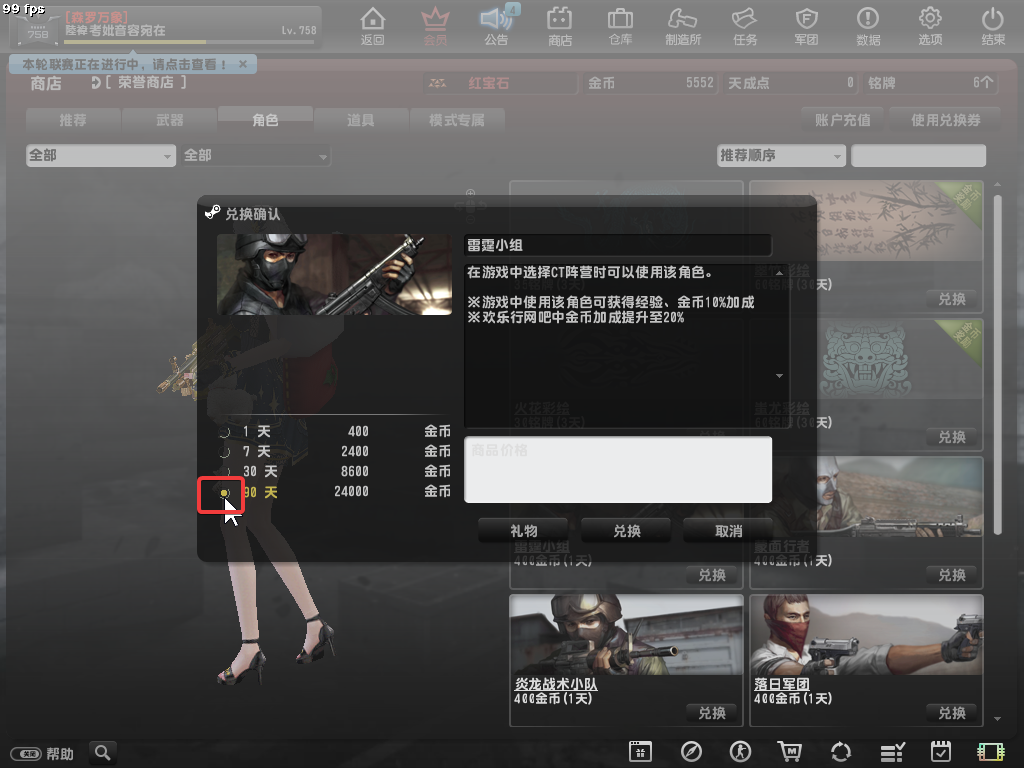
\includegraphics[width=\textwidth]{docs/assets/store_buy_option.png}
    \caption{兑换选项}
    \label{ch4fig-store-buy-option}
\end{figure}
\clearpage

\begin{figure}[H]
    \Centering
    \parbox[l]{\textwidth}{\lstinline{STORE_BUY_X}、\lstinline{STORE_BUY_Y}:点击兑换按钮后弹出的对话框中的“兑换”按钮(图 \ref{ch4fig-store-purchase})。}
    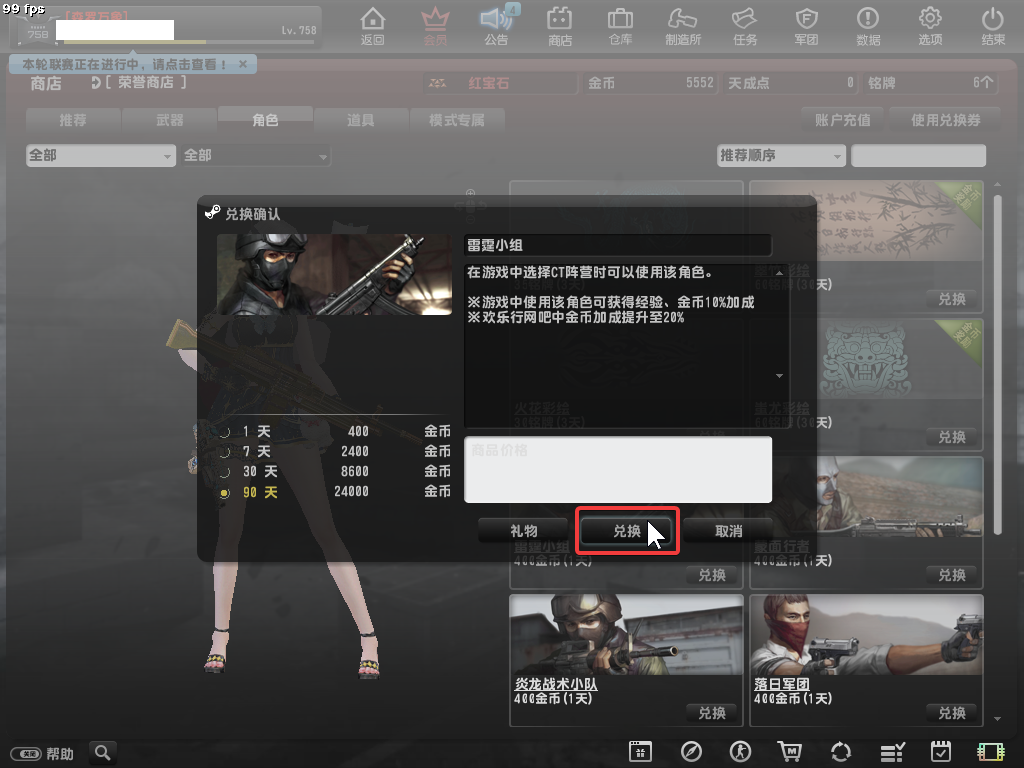
\includegraphics[width=\textwidth]{docs/assets/store_purchase.png}
    \caption{对话框中的“兑换”按钮}
    \label{ch4fig-store-purchase}
\end{figure}
\clearpage

\begin{figure}[H]
    \Centering
    \parbox[l]{\textwidth}{\lstinline{STORE_BUY_CONFIRM_X}、\lstinline{STORE_BUY_CONFIRM_Y}:兑换确认按钮坐标位置(图 \ref{ch4fig-buy-confirm})。}
    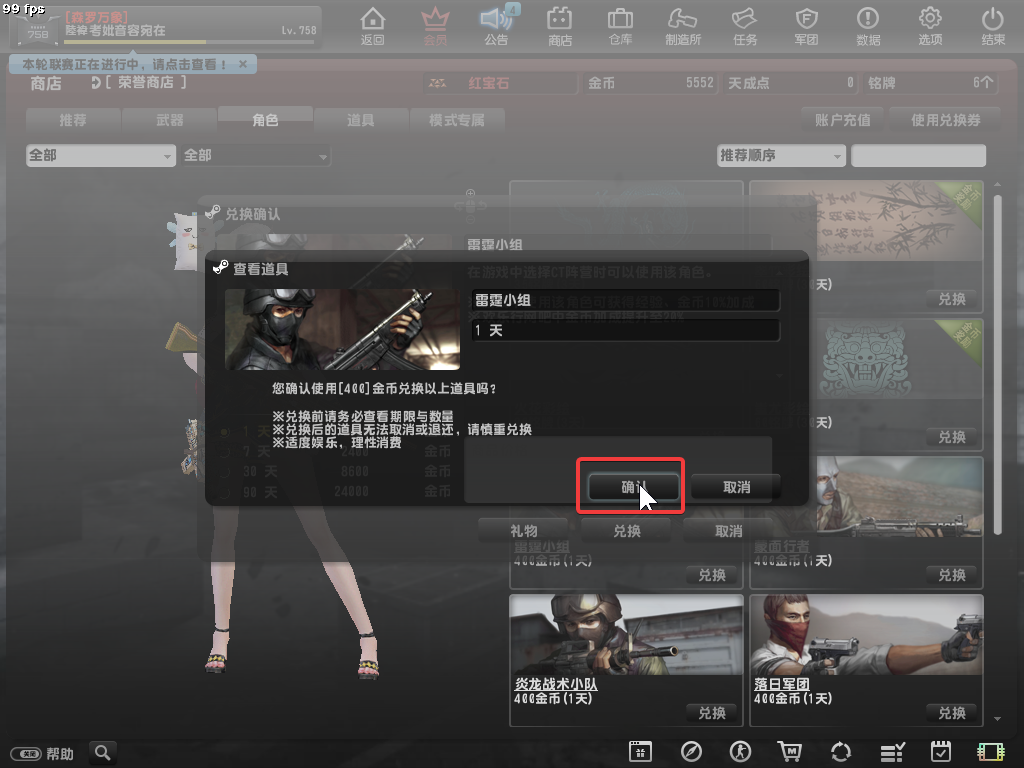
\includegraphics[width=\textwidth]{docs/assets/store_buy_confirm.png}
    \caption{兑换“确认”按钮}
    \label{ch4fig-buy-confirm}
\end{figure}
\clearpage

配置完成后,在罗技控制台中重新保存并运行脚本,以使配置生效。

\subsection{使用方法}

在 0 模式下,将鼠标光标移动到需要购买的物品的兑换按钮处。
随后,切换到 4 模式,购买将自动执行。
切换回 0 模式,购买操作将停止。